
	\begin{figure}
	\centering
	
		\begin{subfigure}[t]{\linewidth}
			\begin{tikzpicture}
%			\node(a){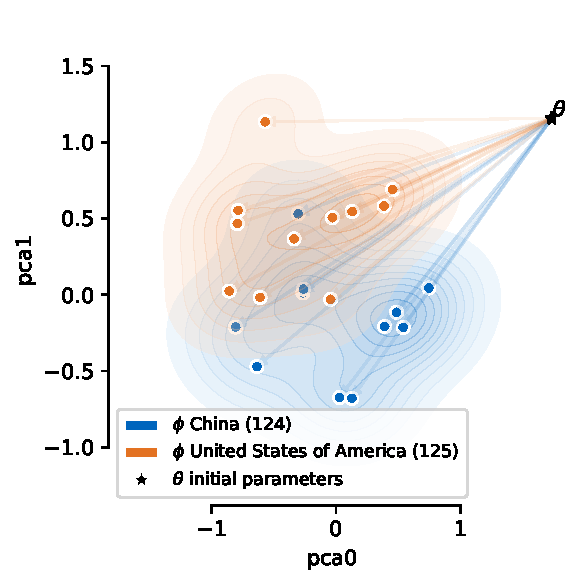
\includegraphics[width=4cm]{figures/sen12ms-adaptation/124-125}};
			\node[]{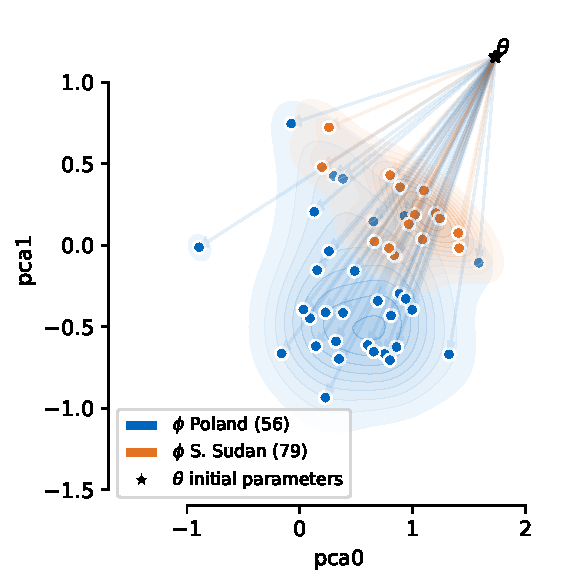
\includegraphics[width=3.8cm]{figures/sen12ms-adaptation/56-79}};	
			\end{tikzpicture}
			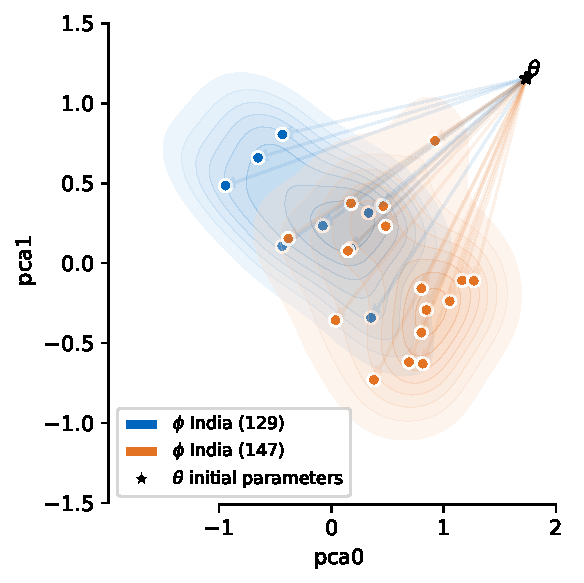
\includegraphics[width=3.8cm]{figures/sen12ms-adaptation/129-147}
			
			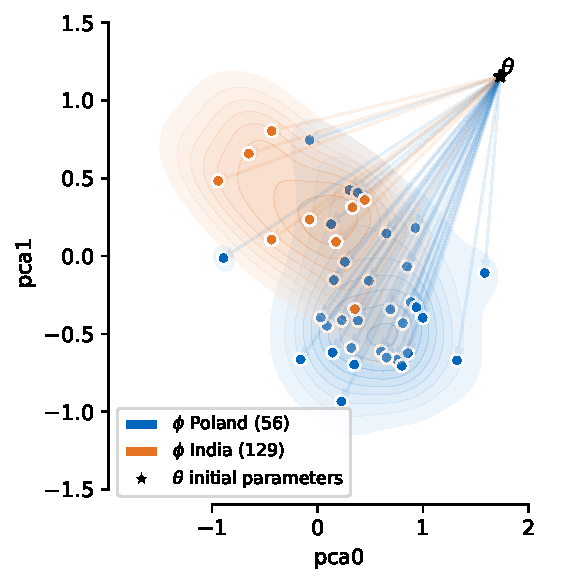
\includegraphics[width=3.8cm]{figures/sen12ms-adaptation/56-129}
			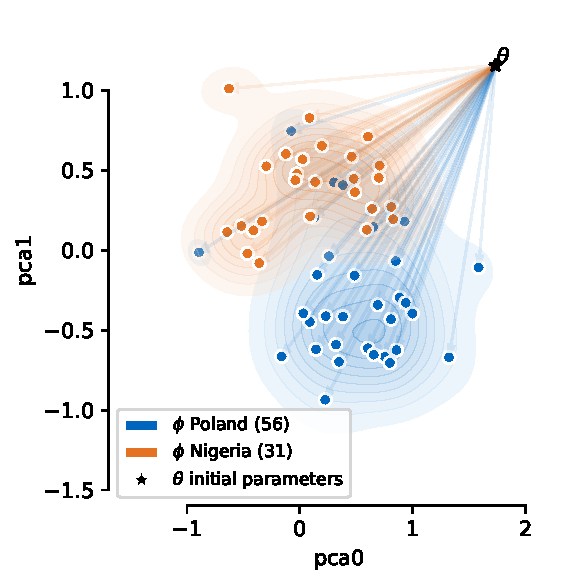
\includegraphics[width=3.8cm]{figures/sen12ms-adaptation/56-31}
			%	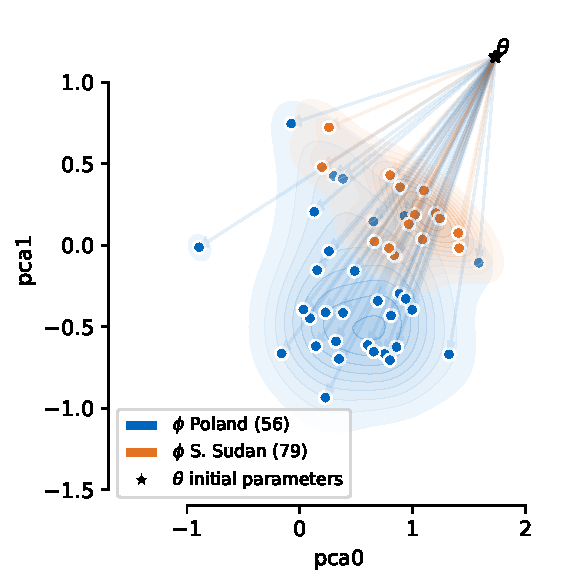
\includegraphics[width=2.5cm]{figures/sen12ms-adaptation/56-79}
			\caption{Adaptation of the MAML-trained CNN model to episodes from different regions.}
		\end{subfigure}
		
		
		\begin{subfigure}[t]{\linewidth}
			\begin{tikzpicture}
			
			\newcommand{\plotloss}[2]{
				\begin{tikzpicture}
				\begin{axis}[
				height=3cm,
				width=\textwidth,
				ymin=0,
				ymax=3,
				title=#2,
				title style={yshift=-.5em},
				ylabel=loss,
				y label style={at={(0.1,0.5)}, font=\sffamily\scriptsize, anchor=center},
				x label style={font=\sffamily\scriptsize, at={(0.5,.15)}, anchor=north},
				title style={font=\scriptsize\sffamily},
				tick label style={font=\tiny\sffamily},
				xlabel=step size $\alpha$,
				ymajorgrids,
				]
				\addplot[tumblue] table [x=step_size, y=testloss0, col sep=comma] {#1};
				\addplot[tumorange] table [x=step_size, y=testloss1, col sep=comma] {#1};
				\addplot[tumblack] table [x=step_size, y=testloss2, col sep=comma] {#1};
				\addplot[tumgreen] table [x=step_size, y=testloss3, col sep=comma] {#1};
				%		\addplot[tumdiagramred] table [x=step_size, y=testloss4, col sep=comma] {#1};
				\end{axis}
				\end{tikzpicture}
			}
			
			\newcommand{\legend}{
				\begin{tikzpicture}[xscale=1.3,yscale=-.5]
				\draw[tumblue, very thick] (0,0) -- node[midway,   above=0.1em, text=black, inner sep=0.01em, font=\sffamily\scriptsize]{query set 1} (1,0);
				\draw[tumorange, very thick] (0,1) -- node[midway, above=0.1em, text=black, inner sep=0.01em, font=\sffamily\scriptsize]{query set 2} (1,1);
				
				\draw[tumblack, very thick] (1.2,0) -- node[midway, above=0.1em, text=black, inner sep=0.01em, font=\sffamily\scriptsize]{query set 3} (2.2,0);
				\draw[tumgreen, very thick] (1.2,1) -- node[midway, above=0.1em, text=black, inner sep=0.01em, font=\sffamily\scriptsize]{query set 4} (2.2,1);
				
				\end{tikzpicture}
			}
			
			\node[anchor=west](a) at (0,0){\plotloss{figures/sen12ms-1d-losses/maml.csv}{MAML}};
			\node[anchor=west](b) at (0,-2.6){\plotloss{figures/sen12ms-1d-losses/pretrained_.csv}{Pretrained}};
			\node[xshift=0em,yshift=-1em, anchor=north east] at (a.north east){\legend};
			
		\end{tikzpicture}
		\caption{1D Loss surface on multiple query sets along the gradient of one support set.}
		\label{fig:1dloss}
	\end{subfigure}
	
% 	\begin{subfigure}[t]{\linewidth}
% 		\tikzstyle{labelstyle} = [font=\tiny\sffamily]
		
% 		\begin{tikzpicture}
		
% 		\newcommand{\traintaska}{
% 			\begin{tikzpicture}[xscale=.75]
% 				\node[label={[labelstyle]below=0em:forest}] at (0,0) {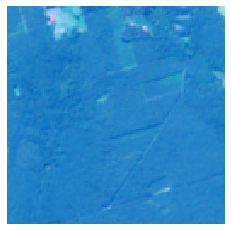
\includegraphics[width=.7cm]{figures/sen12ms-2d-losses/pretrained/0/traintask1/summer-56-Forests-p53br.png}};
% 				\node[label={[labelstyle]below:grassland}] at (1,0) {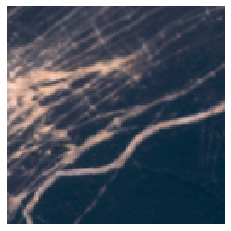
\includegraphics[width=.7cm]{figures/sen12ms-2d-losses/pretrained/0/traintask1/summer-56-Grassland-p37tl.png}};
% 				\node[label={[labelstyle]below:savanna}] at (2,0) {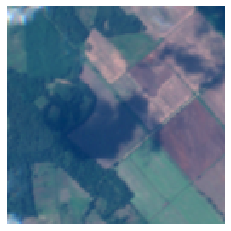
\includegraphics[width=.7cm]{figures/sen12ms-2d-losses/pretrained/0/traintask1/summer-56-Savanna-p168br.png}};
% 				\node[label={[labelstyle]below:urban}] at (3,0) {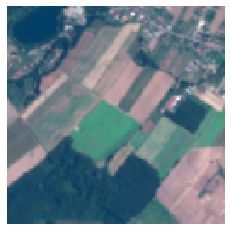
\includegraphics[width=.7cm]{figures/sen12ms-2d-losses/pretrained/0/traintask1/summer-56-Urban_Build-up-p417tl.png}};
% 			\end{tikzpicture}
% 		}
		
% 		\node[label={[font=\scriptsize\sffamily, yshift=-1em]above:MAML}](a){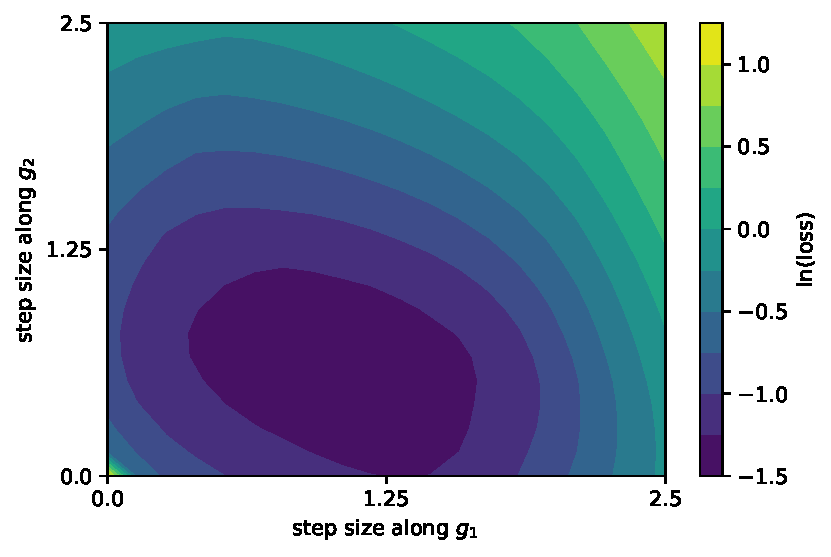
\includegraphics[width=4cm]{figures/sen12ms-2d-losses/maml/0/loss_surface}};
% 		\node[label={[font=\scriptsize\sffamily, yshift=-1em]above:pre-trained}, right=0em of a](pretrained){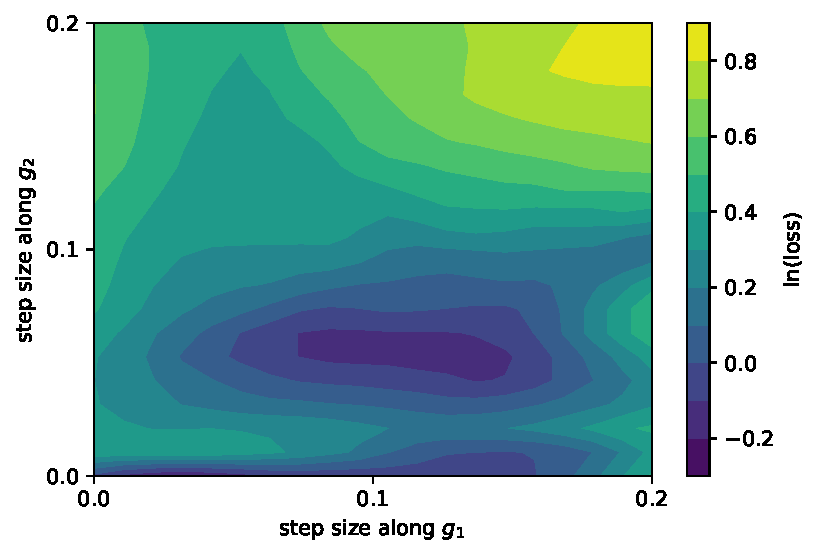
\includegraphics[width=4cm]{figures/sen12ms-2d-losses/pretrained/0/loss_surface}};
% %		\node[below=0em of pretrained]{\traintaska};
		
% 		\end{tikzpicture}
% 		\caption{2D-loss surface on a interpolation between gradients of two support-tasks of the same region and classes}
% 		\label{fig:2dloss}
% 	\end{subfigure}


	\ifdefined\reducecaptionspace
	\setlength{\belowcaptionskip}{-15pt}
	\fi
	
	\caption{The adapted weights $\phi_\tau$ for task $\tau$ vary from region to region (a). The loss surface along the direction of initial weights $\theta$ to $\phi_\tau$ (b) is more convex and allows larger gradient step sizes for model-agnostic meta learning compared to regular pretraining.}
	\label{fig:adaptation}
\end{figure}